% \documentclass{article}
% Tipo di documento. L'uso di twoside implica che i capitoli inizino sempre con la prima pagina a sinistra, eventualmente lasciando una pagina vuota nel capitolo precedente. Se questa cosa è fastidiosa, è possibile rimuoverlo. 
% \documentclass[a4paper, twoside,openright]{report}
\documentclass[a4paper,openright]{report}

\usepackage{graphicx} % Required for inserting images

\usepackage[utf8]{inputenc}

\usepackage{hyperref}

\usepackage{graphicx}
\usepackage{wrapfig}

\usepackage{enumitem}
\usepackage{paracol}
\usepackage{multicol}

\usepackage{geometry}

\usepackage{color}

\usepackage{listings}

\usepackage{amsmath}
\usepackage{bm}

% Uso dei colori
\usepackage[dvipsnames]{xcolor}

\usepackage{tikz}
\usetikzlibrary{automata, arrows}
\usetikzlibrary{positioning}
\usetikzlibrary{shapes.geometric}

\geometry{margin=0.6in}

\setlist[description]{itemsep=0em,topsep=0.5em,parsep=0em}
\setlist[itemize]{itemsep=0em}

\hypersetup{
    colorlinks=true,
    linkcolor=black,
    filecolor=mauve,
    urlcolor=blue,
}

\definecolor{gray}{gray}{0.3}

\newenvironment{notes}{
\par
\color{gray}
\small}

\newcommand{\note}[1]{\begin{notes}{#1}\end{notes}}
\newcommand{\lst}[1]{\lstinline{#1}}
\newcommand{\nl}[0]{\parskip = \baselineskip}

\lstset{frame=false,
 showstringspaces=false,
 breaklines=true;
 columns=flexible,
 basicstyle={\small\ttfamily},
 keywordstyle=\color{blue},
 commentstyle=\color{dkgreen},
 stringstyle=\color{mauve}
 tabsize=3
}

\title{Advanced Software Engineering - Appunti}
\author{Francesco Lorenzoni}
\date{September 2023}

\begin{document}

\maketitle
\tableofcontents

\chapter{Introduction}
\section*{27 - Settembre}
\section{Product based}
In \textit{Project-based SE} there is loop which nowdays cripples software since its early stages of development.
This is due to mutable nature of requirements, which often change throughout time along the features implemented by the software.
\begin{center}
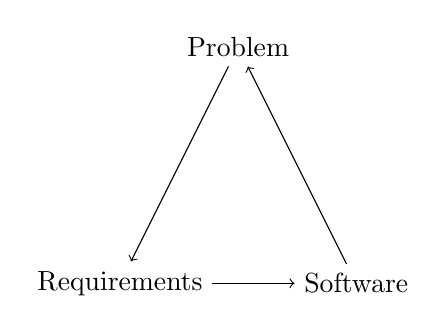
\begin{tikzpicture}
    \node[draw=white,align=left] (A) at (1.5,3) {Problem};
    \node[draw=white,align=left] (B) at (0,0) {Requirements};
    \node[draw=white,align=left] (C) at (3,0) {Software};

    \path [->] (A) edge node[left] {} (B);
    \path [->] (B) edge node[left] {} (C);    
    \path [->] (C) edge node[left] {} (A);    
\end{tikzpicture}
\end{center}

\textit{Product-based SE} is opposed to \textit{Project-based SE} and the above pictures changes as follows.

\begin{center}
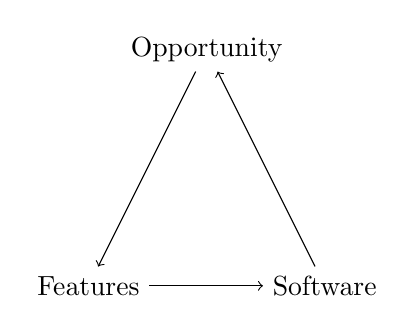
\begin{tikzpicture}
    \node[draw=white,align=left] (A) at (1.5,3) {Opportunity};
    \node[draw=white,align=left] (B) at (0,0) {Features};
    \node[draw=white,align=left] (C) at (3,0) {Software};

    \path [->] (A) edge node[left] {} (B);
    \path [->] (B) edge node[left] {} (C);    
    \path [->] (C) edge node[left] {} (A);    
\end{tikzpicture}
\end{center}

\section{Agile}
Agile is a collection of principles and methods applied in the software development field.
\nl

Opposed to project-based SE, in Agile the client is requested to express the requirements not in technical terms but in features.

Agile suggests an incremental development model

\subsection*{Principles}
\begin{enumerate}
    \label{subsec:agile_principles}
    \item Satisfy customer through early and continuous delivery of valuable software
    \item Welcome changing requirement, even late in development.
    Agile processes harness change for the customer's comptetitive advantage
    \item Deliver working software frequently, from a couple of weeks to a couple of months, with a preference to the shorter timescale
    \item Business people and devs must work together daily throughout the prokect
    \item Build porjects around motivated individuals and give them the environment and support they need
    \item The most efficient and effective method of conveying information to and within a dev team is face-to-face conversation
    \item Working software is the primary measure of progress
    \item Agile processes promote sustainable dev 
    \item Continuous attention to technical excellence and good design enhances agility
    \item Simplicity i.e. art of maximizing the amount of work not done is essential
    \item The best architectures, requirements, and designs emerge from self-organizing teams.
\end{enumerate}

Extreme Programming was proposed as part of the agile methodology

\section{Scrum}
Since requirements changes are rather frequent, long-term plans are unreliable,
hence SE aims to formulate short-term plans.

Scrum is found on \textbf{empiricism} and \textbf{lean thinking}; it asserts that knowledge comes from experience, and that decisions should be made on observations.

Other key terms are code \textbf{Transparency} among the team and with the customer, \textbf{Inspection} of produced code and software (artifacts), \textbf{Adaptation} to changes in features and requirements.

The \textbf{Scrum Team} is composed by:
\begin{enumerate}
    \item \textbf{Product Owner}: must ensure that the dev team is always focused on the goal
    \item \textbf{Scrum Master}: Scrum expert which drives the team to apply properly the Scrum framework.
    \item \textbf{Developers}: actual monkeys people which write code
\end{enumerate}

In scrum SW is developed in \textbf{sprints}, i.e. fixed-length periods with a specific goal to be achieved.

\begin{itemize}
    \item Product backlog: to-do list of items to be implemented
    \item Timeboxed sprints
    \item Self-organizing teams
\end{itemize}

...
\textbf{Prod Backlog Revised}\\
\textbf{PBI Estimation Metrics}

\subsection{Timeboxed Sprints}
Even if at the end of a srpint the goal hasn't been reached, "no worries", the work stops anyway;
there will be a new sprint which will include the work which has not been implemented in the previous one.

\subsection{Scrum Meetings}

\subsection{Agile activities}
Test automation
Continuous integration

\subsection{Sprint reviews}
At the end of each sprint there is a review meeting which involves the \textit{whole} team.
The \textit{product owner} has the ultimate authority to decide wether the sprint goal has been reached or not.
The sprint review should include a process review, in which the whole team shares ideas on how to improve their way of working.

\textbf{Team size}\nl

\section{5 - Ottobre}



\chapter{IEEE 802.11}

\begin{figure}[htbp]
   \centering
   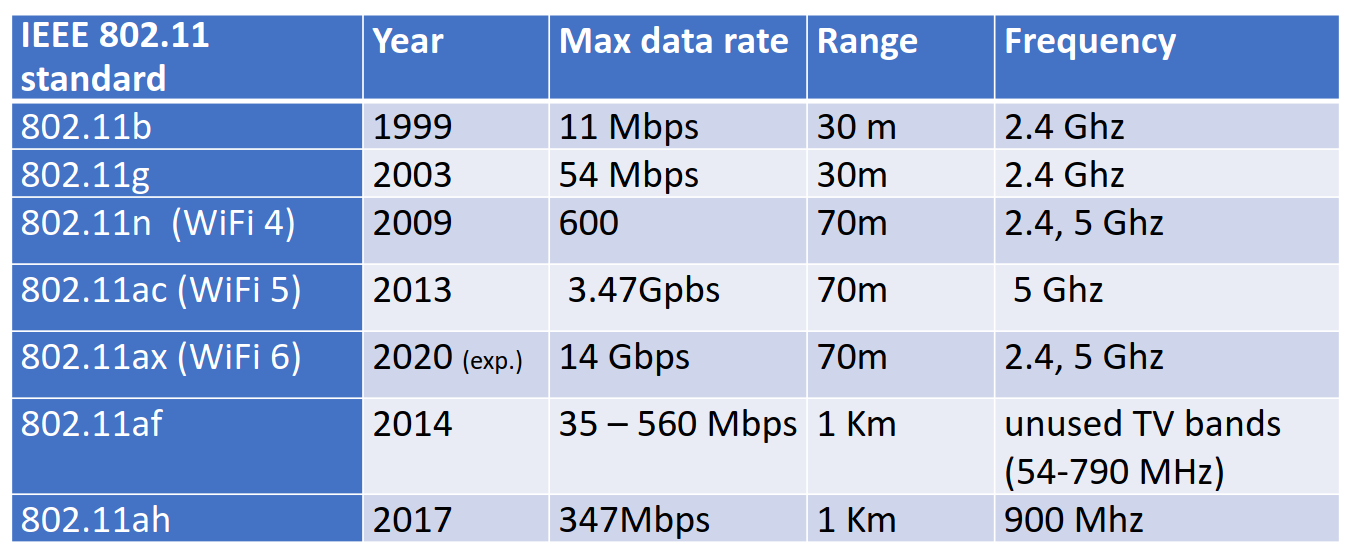
\includegraphics{images/ieee_bgn.png}
   \caption{IEEE 802.11 standards}
   \label{fig:ieee_bgn}
   All these standards \texttt{use \texttt{CSMA/CA} for multiple access}, and have base-station and ad-hoc network versions
\end{figure}

IEEE 802.11 standards refer to the \textit{Physical} Layer.
In case of an AP (Access Point), every station must channel its communication through the AP to talk to any other. Otherwise, in an \textit{Ad-Hoc} network, stations can communicate directly with each other.

TODO

\note{TODO non ci sono domande su questa cose nel pdf}
\chapter{Fabric}
``Fabric'' is the term used to refer to the \textit{interconnection} between nodes of a datacenter.\\
\ul{Cabling is of paramount importance.}
\note{Prof. Cisternino learnt it ``the hard way'' when he performed the cabling of the first UniPi datacenter by himself}
\begin{enumerate}
   \item Maintenance
   \item Cooling
   \begin{enumerate}
      \item Cables may heat up
      \item Cables may obstruct air flow
   \end{enumerate}
   \item Determines which machines interact with each other (\textit{fabric})
   \item Bandwidth
   \item Not neglectable cost
\end{enumerate}

We refer to North-South traffic indicating the traffic outgoing and incoming to the datacenter (internet), while we refer to East-West as the internal traffic between servers.
Most of the network (or fabric) traffic is processed horizontally (North-South traffic)\footnote{Seems odd that ``horizontal'' refers to North-South traffic, but that's how it is.}.


\section{Bandwidth and Storage implications}
\label{sec:bandwidth_storage}
A standard datacenter has servers connected with 25Gbit links in both directions, summing up to 50Gbit total bandwidth.
Current SSDs using NVMe provide much more, about $3.5 GB/s$, making \ul{4 drives are enough to saturate a 100Gbit/s link.}\\
We moved from a situation where the \textbf{bottleneck} were slow Hard Drives, to the current one where the bottleneck is the ---network--- \textbf{bandwidth}.\\
Recently the PCI 3.0, which lasted very long ---providing roughly$\sim\texttt{120Gbit/s}$ using 16 pin---, suddenly become unsufficient to handle the needed traffic.

Considering this, \ul{datacenters must be designed to allow \textit{Terabytes} of data to be moved in east-west traffic.}

\begin{center}
   \ul{\textit{The \textbf{fabric} is the glue that makes the datacenter possible.}}
\end{center}

Besides, a single server is \textit{unable} to handle 10TBs of data and handling requests from 3000 users simultaneously. It is necessary to \textbf{distribute} the requests.

HDDs are still currently used for \textbf{cold storage};
CPUs will access data exclusively from SSDs, and sometimes the server is shipped with on board \textbf{full-flash storage}.\\
The difference in price between SSDs and HDDs becomes negligible since you pay for top CPU, top GPU, top RAM;
furthermore, you can't waste ---the high amount of--- energy ---consumed by such components--- by waiting for a slow drive.

SSDs have a known write limit, but today, the usually last enough time: if you write the whole disk every day it will last for 5 years. Most-likely after five years you'd have to renew some components anyway, besides the failure is a predictable event.

\section{Cables and standards}
\subsection{Optical}
Electric current propagates at a speed $s = {\sim}0.6c$.
Hence \textbf{optical fiber} is ---at least in theory?--- faster.

\textbf{Lasers} are a coherent beam of equal fotons. It is possible to transfer energy through such fotons. Something resembling a laser is used for optical fibers.

Blu-Ray came out when scientists managed to create light using frequencies in the Blu area, which are the higher ones.
Currently, the best and most expensive optical fibers exploit blu-lasers as source of light.

Note that with optical you always need 2 fibers, one sending and the other receiving. The two possible connectors are \texttt{SC} and \texttt{LC}.
Sometimes the two ends of the cable are detachable so that the cables may be switched; this is useful because sometimes you may want to attach the TX cable on the RX plug and viceversa. 

\begin{figure}[htbp]
   \centering
   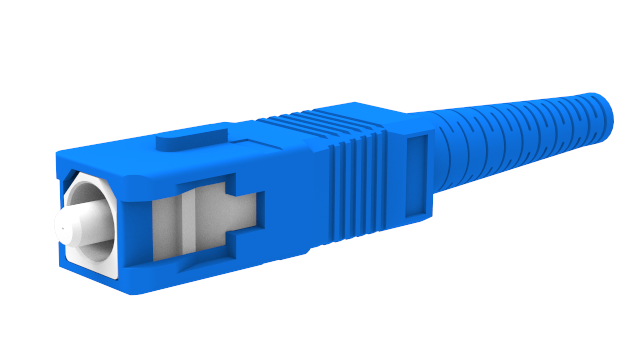
\includegraphics[width=0.25\columnwidth]{images/SC.png}
   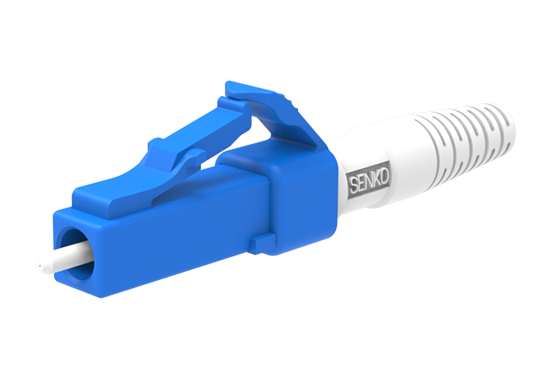
\includegraphics[width=0.25\columnwidth]{images/LC.png}
   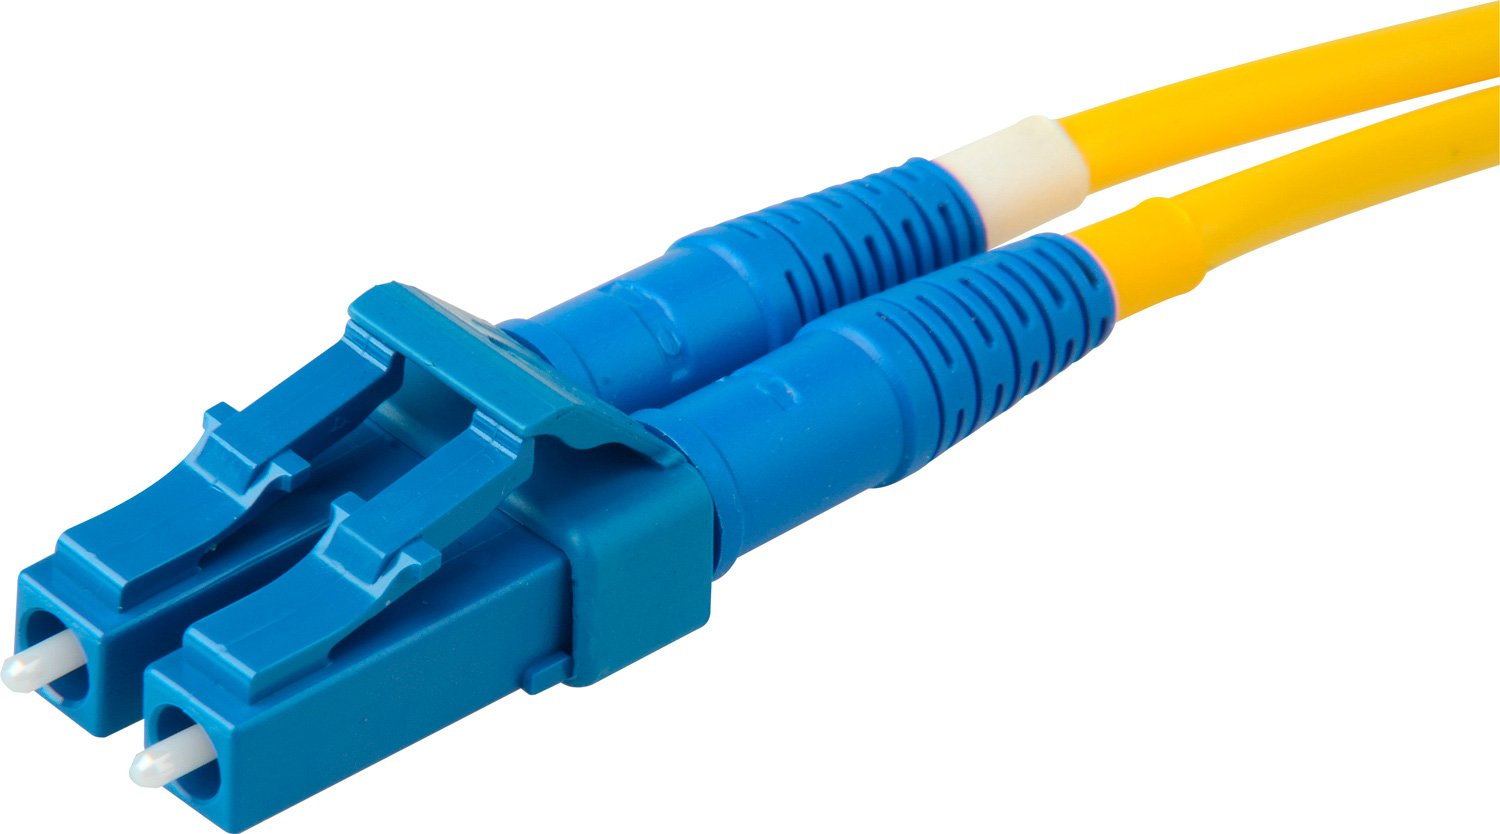
\includegraphics[width=0.25\columnwidth]{images/LC_coupled.JPG}
   \caption{\texttt{SC} and \texttt{LC} connectors}
   \label{fig:sc_lc_connectors}
\end{figure}

\subsection{Copper wires}
In case of electricity there are many aspects to be considered. Interferences, cable diameter/size, length, and also the fact that if a \texttt{1} has been transmitted for some time, it takes longer to transmit a \texttt{0}, due to the \textit{commutation} that must happen.
\nl

\begin{paracol}{2}
   \colfill
   \textbf{RJ45} is a standard physical interfaced for copper wires, which allows up to 1Gbit regularly.
   The \texttt{Cat 7} cables still use the RJ45 as connector and provide instead 10Gbit/s, but are very uncomfortable, they are so thick that they are difficult to bend.
   
   It is estimated that there have been installed $70 \times 10^9m$ of Ethernet cables, making them the most used.
   \colfill
   \switchcolumn

   \begin{figure}[htbp]
      \centering
      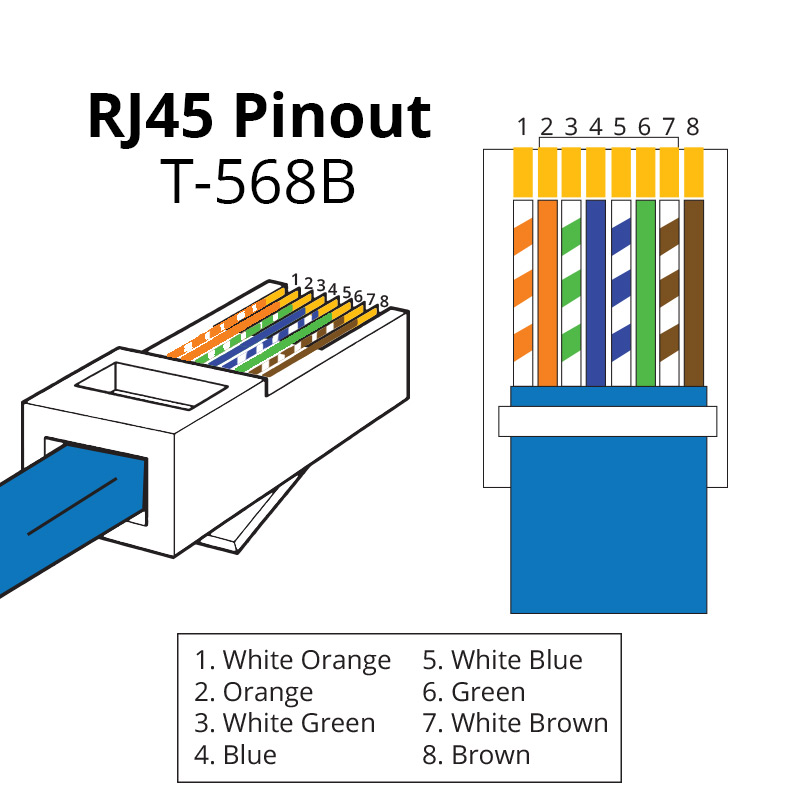
\includegraphics{images/RJ45_T568B.jpg}
      \caption{RJ45 - T568B}
      \label{fig:RJ45_T568B}
   \end{figure}
\end{paracol}

\subsection{SFP - Small Form-factor Pluggable}
There can be a cable with a LC in one side and a SC on the other side.
Instead of making switches with the optical plugs, switches were created with electrical plugs that would be able to host a \textbf{standard transceiver}.
The latter is a pluggable module that will receive current power and electrical signals for the transmission, which is responsible for transitioning between electrical signals and Optical signal (and viceversa).

\begin{paracol}{2}
   
   The aim of SFP is to decouple the optical transceivers from the server modules.
   \note{Is this correct?}
   They allow to go \textit{optic-copper}, \textit{copper-optic}, \textit{optic-optic} and \textit{copper-copper}.\\
   SFP and GBIC (oldest one, now dead) pluggable modules acting as active transceivers for optical wiring using RJ45 connector.\\
   \ul{A single cable having SFP ends costs about 100€}.
   The cost ain't neglectable \smiley.
   \note{\begin{itemize}
      \item[\texttt{SFP}] $\longrightarrow 1Gbit $
      \item[\texttt{SFP+}] $\longrightarrow 10Gbit $
      \item[\texttt{SFP28}] $\longrightarrow 25Gbit$
      \note{This is the current standard}
      \item[\texttt{QSFP28}] $\longrightarrow 4\times25Gbit$
   \end{itemize}}


   \switchcolumn

   \begin{figure}[htbp]
      \centering
      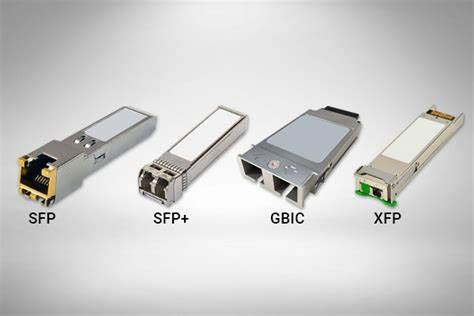
\includegraphics{images/sfp.jpeg}
      \caption{SFP transceivers form factors}
      \label{fig:sfp}
   \end{figure}
\end{paracol}

\note{Fun fact: ci sono 9 cavi USB-C e solo due portano informazioni video.}

\subsubsection{Issues about cabling and fabric}
The key point is that it would be desirable for cabling to be reconfigurable, that's why transceivers are so important.

\note{There are things called \textit{``Muffole''}, which are used for joining optical fiber cables, allowing for longer distances to be covered.
They are designed to be underground.}

Data traffic is always at least SFP+.
Current standard is SFP28. Various SFP are typically compatible, the shape of the plug should stay the same.
On switches there also some ports which are \texttt{QSFP+} or \texttt{QSFP28}, which allow up to \texttt{40} and \texttt{100Gbit/s} respecitively, and are used for north-south traffic.
\note{The \texttt{Q} letter stands for \textit{Quality}}

Switches for datacenters should be \textbf{non-blocking}, meaning that no port has to wait for other ones ---or any other thing--- before transmitting, they can also transmit simultaneously.


\ul{In every datacenter it is \textit{MANDATORY} to document the cabling.}

\subsection{InfiniBand}
Even though Ethernet is famous, it is not the only standard. InfiniBand is another one, which is used in supercomputers and known for its very high throughput and very low latency ($\sim 2\mu s$).
It may send messages up to 2GB each, with 16 priority levels.
It is a \textit{lossless protocol}, meaning that if a packet is received, its integrity is guaranteed.

\textit{IB} avoids TCP/IP stack, which is very heavy, and instead uses MPI (\textit{Message Passing Interface}), which is a way to distributed parallel programs, also exploited by OmniPath.

InfiniBand cables and connectors look similar to Ethernet ones, but they are not compatible.

Aside from HPC environments, it is uncommon to build an entire network with InfiniBand, typically there is an IB switch to whom the servers equipped with IB NICs are connected, which intereacts with the rest of the network with Ethernet, because ``it's cheaper and it works''.
\note{Today, we are about 400 Gbit/s on both IB and Ethernet.}

\subsection{RDMA - Remote Direct Memory Access}

RDMA is a technology API based (not a protocol!) that allows to access memory of a remote machine without involving the CPU or the OS of the remote machine.

RDMA supports zero-copy networking by enabling the network adapter to transfer data directly to or from application memory, eliminating the need to copy data between application memory and the data buffers in the operating system.\\
The main use case is distributed storage.

RoCE (\textit{RDMA over Converged Ethernet}) is a network protocol that allows remote direct memory access (RDMA) over an Ethernet network.

\subsection{Omni-Path}
Omni-Path is a high-performance computing network architecture, developed by Intel. It is a successor to Intel's InfiniBand, and competes with InfiniBand's EDR and HDR technologies.

Intel plans to develop technology that will serve as the on-ramp to \textit{exascale computing}\footnote{A computing system capable of the least one exaFLOPS}, which is the next frontier in high-performance computing.


\chapter{BitTorrent}

The goal of \textit{Content Distribution Networks} is to distribute web contents to hundreds of thousands or millions
of simultaneous users, \ul{exploiting data and/or service \textbf{replication} on different \textbf{mirror servers}}.

In \textbf{P2P CDN} the initial file request are served by a centralized server, and further requests served by peers which have already received and replicated the files (\textbf{\textit{seeders}}), without involving the initial server.

\begin{center}
\fbox{
   \begin{minipage}{0.8\columnwidth}
      \nl
      \begin{center}
         \ul{\textbf{BitTorrent} in a nutshell}
      \end{center}
      \nl

      \begin{itemize}
         \item Basically a \textit{Content Distribution Network} (\texttt{CDN})
         \item A distributed set of hosts cooperating to distribute large data set to end users.
         \item Efficient content distribution systems using \textit{file swarming}
         \item Does \textit{not} perform all the functions of a typical P2P system, like searching
         \item Rather than providing a search protocol itself, was designed to integrate seamlessly with the Web and made file descriptors available via Web, which could be searched with standard Web search
         \item \textit{File swarming}: a peer makes whatever portion of the file that is downloaded immediately available for sharing
      \end{itemize}
   \end{minipage}  
   }
\end{center}

\section{Deeper into BitTorrent}
\begin{figure}[htbp]
   \centering
   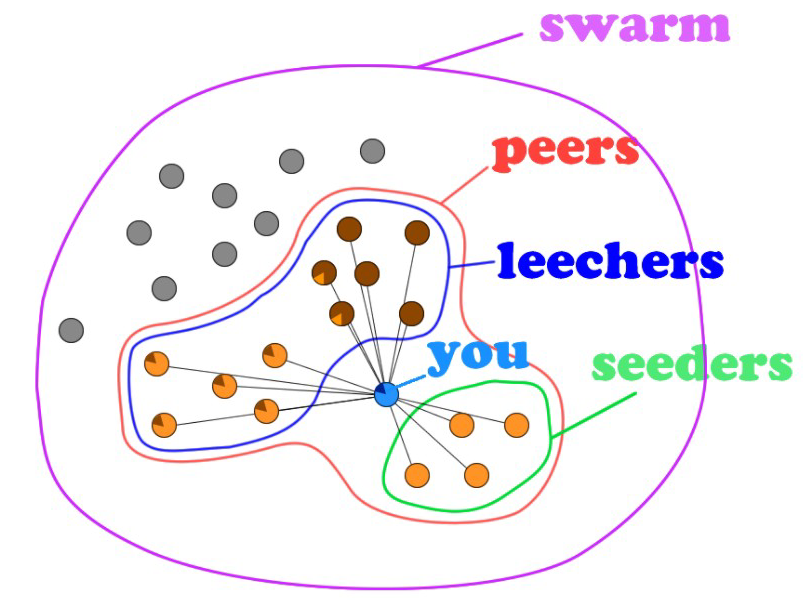
\includegraphics{images/bit_swarmschema.png}
   \caption{Swarm schema}
   \label{fig:bit_swarmschema}
\end{figure}
\subsection{Glossary}
\begin{itemize}
   \item \textbf{tracker}: active entity which coordinates
   the peers sharing the file, taking trace of who is currently providing the content
   \note{\begin{itemize}
      \item Joe connects to the tracker announcing the content
      \item the tracker now knows Joe is providing the file
   \end{itemize}}
   \item \texttt{.torrent} a descriptor of the file to be published on a server, which includes a reference to a tracker
   \item \textbf{swarm} set of peers collaborating to the distribution of the same file coordinated by the same tracker
   \item \textbf{seeder} peer which owns all the parts of the file
   \item \textbf{leecher} peer which has some part or no part of the file and downloads the file from the seeders and/or from other lechers.
\end{itemize}

\subsection{Protocol Overview}
\begin{figure}[htbp]
   \centering
   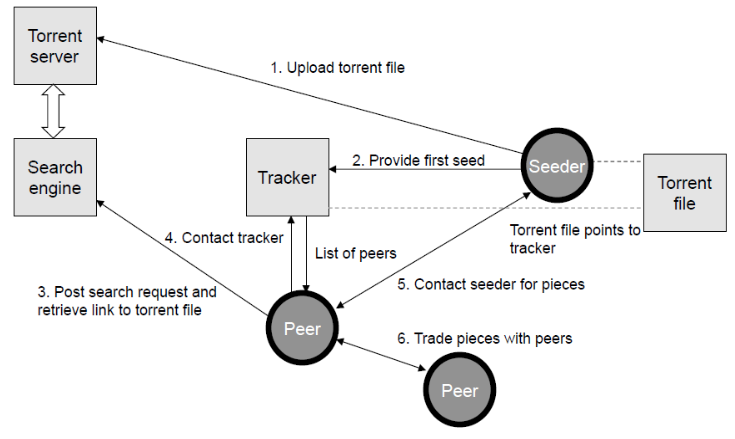
\includegraphics{images/bit_overview.png}
   \caption{BitTorrent protocol overview}
   \label{fig:bit_overview}
   BitTorrent protocol is built on top of HTTP
\end{figure}
\labelitemize{\textit{Seeder}}{
   \begin{enumerate}
      \item Upload the .torrent on a Torrent Server
      \item Opens a connection to the Tracker and informs it of its own existence: for the moment, it is the only peer which owns the file
   \end{enumerate}
}
\labelitemize{\textit{Peers}}{
   \begin{enumerate}
      \setcounter{enumi}{2}
      \item Retrieves the file descriptor (.torrent) and opens it through the BitTorrent
      client
      \item Opens a connection to the tracker and informs it of its own existence and
      receives from the tracker a list of peers of the swarm
      \item Opens a set of connections with other peers of the swarm.
   \end{enumerate}
}

Objects are serialized in \textbf{Bencode}, which is ---not popular as \texttt{JSON}--- used only in torrent; provides 4 data types: String, Integer, Lists and Dictionaries.\\
Content is split into chunks called pieces (256KB - 2MB):
when a peer receives a piece, it becomes the seeder of that piece.
\note{
   \ns
      There is a SHA-1 hash per piece stored in the .torrent file, used to check the piece once it is fully downloaded, 
      allowing to require retransmission in case the check fails.\\
      Pieces size got adapted to have a reasonably small .torrent file
}
Pieces are then split in \textbf{subpieces} (\textit{\textbf{blocks}}) of 16KB, with each one downloadable from a different peer, optimizing the bandwith and allowing \textit{pipelining}, decreasing the overall download time.

Trackers keep a database of swarms identified by torrent hash, and knows also the state of each peer in each swarm.
In the last versions, \textbf{trackerless} BitTorrent uses \textit{Kademlia DHT} to avoid the centralization point of the tracker.

\section{Pieces selection}
The order in which pieces are selected by different peers is critical for good performance, to avoid making peers end up stuck with the same pieces.
\labelitemize{\textit{Policies}}{
   \begin{itemize}
      \item \textbf{Strict Priority}\\
      Complete the ``assembling'' of a piece before asking for another piece
      \item \textbf{Rarest First}\\
      Download the rarest pieces first
      \item \textbf{Random First Piece}\\
      Choose a random piece ---only--- in the bootstrap phase
      \item \textbf{Endgame}\\
      When the file download is almost terminated, the remaining pieces are required in \textit{parallel} to all peers who own them.
      This policy is executed for a small period of time
   \end{itemize}
}

\subsection{Free Riders}
Free riders in BitTorrent are peers that do not put their bandwidth at disposal of the community.\\
Several non official BitTorrent clients enable the user to limit the upload bandwidth as they like.

However, an approach to solve this problem is based on \textbf{reciprocity}, allowing a client to obtain a good service if and only if it gives a good service to the community, by exploiting a dynamic strategy based on connection monitoring called ``Tit for Tat'', implemented using \textbf{choking}:\\
choking means \textit{temporarily} refusing to upload to another peer, but still downloading from them;  
the principle is to upload to peers who have uploaded to us.

\labelitemize{\textit{Choking}}{
\begin{center}
   \textit{The local peer can receive data from a remote peer if}
   \begin{itemize}
      \item The local peer is \textit{interested} in the remote peer
      \item The remote peer \textit{unchoked} the local peer
   \end{itemize}
\end{center}
   }

Choking only peers that upload the most to the local peers would lead to ignoring peers that recently join the network
and to the lack of discovery of connections actually better than the used ones.\\
To avoid this, BitTorrent uses \textbf{optimistic unchoking}, i.e. \ul{one random peer is being unchoked}.\\
Then, every 30s an interested and choked peer is selected at random \textbf{planned optimistic unchoke} (\texttt{POU}), and if this new connection turns out to be better than one of the existing
unchoked connections, it will replace it.

In case a peer is chocked by everyone, it follows an \textbf{anti-snubbing} policy, by increasing the number of simultaneous optimistic
unchocke to more than one.

For \textit{seeders} this schema does clearly not apply, since they do not have to download anything; hence they use a different choking algorithm:
\ul{unchoke peers with the highest upload rate}, ensuring that pieces get uploaded and replicated faster.

\section{DHT and BitTorrent}
Kademlia is the protocol used by the largest public DHTs.
Bittorrent Inc. introduces its own DHT, called \textit{Mainline DHT}.
With respect to Kademlia there are some improvements concerning 
\begin{itemize}
   \item Routing table management
   \item Look-up
\end{itemize}

The main purpose of Mainline DHT is to provide a “trackerless” peer discovery mechanism to locate peers belonging to a swarm.

\end{document}
